\newpage
\section{Particle Characterization and Tracking Using Optical Interferences}
\label{sec:chapter2}

\subsection{Introduction}

Properties of coherent light to produce interference has been widely deployed in metrology for a long time as illustrated by, for example, the famous Fabry-Pérot  \cite{fabry_theorie_1899, perot_application_1899} and Michelson interferometers \cite{michelson_relative_1887}. The latter was initially used to evaluate the rotation of the Earth and is still employed today for the recent measurement of gravitational waves
\cite{ligo_scientific_collaboration_and_virgo_collaboration_gw151226_2016}. 
Since the beginning of the century, interest on tracking and characterizing colloidal particles risen thanks to the democratization of micro fluidics and lab-on-a-chip technologies. In the following, I will provide some insights on the three most used tracking methods:

\begin{itemize}
	\item Reflection Interference Contrast Microscopy (\gls{RICM})
	\item Lorenz-Mie theory
	\item Rayleigh-Sommerfeld back-propagation
\end{itemize}

The first one, \gls{RICM}, uses the principle of optical-path difference in a Michelson interferometer. The other two, use the interferences between the light scattered by the colloid and the incident light. Generally, both sources are collinear, so that we speak of in-line holography. 



\subsection{Reflection Interference Contrast Microscopy}




\gls{RICM} was first introduced in cell biology by Curtis to study embryonic chick heart fibroblasts \cite{curtis_mechanism_1964} in 1964. \gls{RICM} gained in popularity 40 years after both in biology and physics \cite{filler_reflection_2000, siver_use_2000, weber_2_2003, limozin_quantitative_2009, nadal_probing_2002, raedler_measurement_1992}. It was also used recently in soft matter physics to study the elastohydrodynamic lift at a soft wall \cite{davies_elastohydrodynamic_2018}.

When we illuminate a colloid with a plane wave from the bottom, a part of the light is reflected at the surface of the glass substrate and another part, at the colloid surface. The difference of optical paths between two reflections creates an interference pattern. Let us focus on the mathematical description of this phenomenon. In the far field, we can describe two one-dimensional electric field vectors with same angular frequency $\omega$ \cite{f_bohren_absorption_1998} as propagative waves, through:

\begin{equation}
	\vec{E}_1(\vec{r}, t) = \vec{E}_{0_1} \cos(\vec{k}_1 \cdot \vec{r} - \omega t + \epsilon_1) ~,
\end{equation}
and:
\begin{equation}
	\vec{E}_2(\vec{r}, t) = \vec{E}_{0_2} \cos (\vec{k}_2 \cdot \vec{r} - \omega t + \epsilon_2) ~,
\end{equation}


\nomenclature{$\vec{E}$}{Electrical field}
\nomenclature{$k$}{Wave number}
\nomenclature{$\omega$}{Pulsation}

where the $k_i$ are the wave vector satisfying $|\vec{k_i}|=k =2\pi n_{\mathrm{m}}/\lambda$, the angular wavenumber, $\lambda$ being the illumination wavelength, $n_\mathrm{m}$ the optical index of the medium, $\epsilon_{1,2}$ the initial phases of each wave and $\vec{r}$ the position. Here, the origin ($\vec{r} = \vec{0}$) is taken at the position of the first reflection (\textit{i.e.} the glass slide). Thus, on the particle, $\vec{r}$ is given by the particle's height such that $|r| = z$. 

\begin{figure}[H]
	\centering
	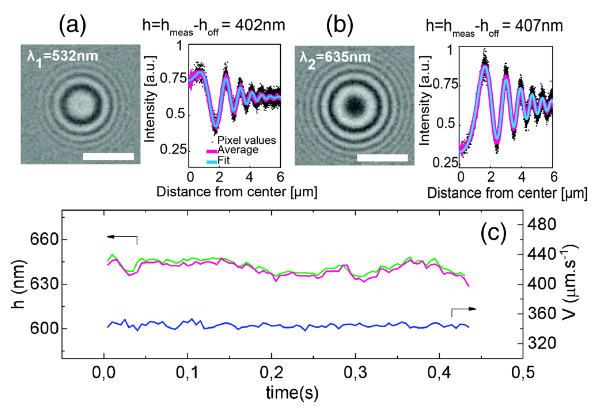
\includegraphics[scale=1]{02_body/chapter2/images/RICM.png}
	\caption{Figure from \cite{davies_elastohydrodynamic_2018} representing \gls{RICM} with two wavelengths. (a) Left: interference patterns created with a wavelength $\lambda_1 = 532$ nm (scale bar $ 5~\mathrm{\mu m}$). 
		Right: radial intensity profile (black dots) extracted from the image, azimuthally averaged (magenta line) and fitted with Eq.\ref{Eq.RICM} to measure the height of the particle (here noted $h$). (b) Same as (a) with a wavelength $\lambda_2 = 635$ nm. (c) Time series of the height $h$ of a particle  (green: $ \lambda_1$, purple: $\lambda_2$) and the particle velocity measured along the flow (in blue). }
	\label{fig.RICM}
\end{figure}


Experimentally, one measures the intensity of the interference patterns. They can be computed from the time-averaged squared total electric field $\vec{E} = \vec{E}_1 + \vec{E}_2$. The measured intensity is thus given by:

\begin{equation}
	\begin{aligned}
		I & = \langle \vec{E}^2 \rangle = \langle \vec{E}_1^2 + \vec{E}_2^2 + 2\vec{E}_1 \cdot \vec{E}_2 \rangle 
		= \langle \vec{E}_1^2 \rangle + \langle \vec{E}_2^2 \rangle  + 2 \langle \vec{E}_1 \cdot \vec{E}_2 \rangle  ~,\\
	\end{aligned}
\end{equation} 

where $ \langle \vec{E}_1^2 \rangle $ and  $\langle \vec{E}_2^2 \rangle$ are respectively given by $I_1$ and $I_2$, the incident intensities. Using trigonometry, we have:

\begin{equation}
	\left\langle  
	\vec{E}_1 \cdot \vec{E}_2 \rangle = 
	\langle
	\frac{1}{2} \vec{E}_{0_1}  \vec{E}_{0_2} 
	\left[
	\cos 
	\left(
	\vec{k}_1 \cdot \vec{r} - \vec{k}_1 \cdot \vec{r} + \phi 
	\right) 
	+ 
	\cos
	\left(
	2\omega t + \phi'
	\right)
	\right]
	\right\rangle_t~.
\end{equation}

As we average over time, the second cosine vanishes. Thus one has:

\begin{equation}
	\langle \vec{E}_1 \cdot \vec{E}_2 \rangle = \frac{1}{2} \langle  \vec{E}_{0_1}  \vec{E}_{0_2} \rangle
	\cos 
	\left(
	\vec{k}_1 \cdot \vec{r} - \vec{k}_2 \cdot \vec{r} + \phi 
	\right)  ~,
\end{equation}

with $\phi$ the phase difference between the two fields, which is usually equal to $\pi$ due to the reflection properties on a higher optical index. Indeed, a colloid has generally a greater optical index than the dilution medium.  Finally, the total intensity can be read as:


\begin{equation}
	I = I_1 + I_2 + 2 \sqrt{I_1 I_2} 
	\cos 
	\left(
	\vec{k}_1 \cdot \vec{r} - \vec{k}_2 \cdot \vec{r} + \phi 
	\right) ~.
\end{equation}

By taking $k_1 = - k_2$ due to the reflection properties, we have:


\begin{equation}
	I = I_1 + I_2 + 2 \sqrt{I_1 I_2} 
	\cos 
	\left(
	\frac{4 \pi n_{\mathrm{m}}}{\lambda} z + \phi 
	\right) ~.
\end{equation}


So far we supposed that the reflection occurs at a unique point; however, we would likely be using spherical colloids. Therefore, illuminating from the bottom, the reflection happens on half of the sphere surface. Moreover, thanks to the spherical geometry the holograms exhibit a radial symmetry, we thus write one can write the radial interference intensity $I(x)$, with $x$ the distance from the pattern center, through \cite{ raedler_measurement_1992}:


\begin{equation}
	I(x) = A_0 + A_1 \mathrm{e}^{-b_1 x^2} + A_2^{-b_2 x^2} \cos \left[ \frac{4\pi n_m}{\lambda}\left( g(x) + z \right) + \phi \right] ~,
	\label{Eq.RICM}
\end{equation}

Where $A_1$ and $b_1$ are parameters \cite{raedler_measurement_1992} that fit the slightly bent background that arises from diffuse reflection on the upper part of the sphere, $A_2$ and $b_2$ the decaying contrast of the higher order maxima, $A_0$ background intensity, and

\begin{equation}
	g(x) = a - \sqrt{a^2 - x^2} ~,
\end{equation}

is the sphere profile, to consider  the increase sphere-wall as $x$ increases.
Finally, this method benefits from equations that are computationally light and enable a quick tracking of particles. However, as we can see in Eq.~(\ref{Eq.RICM}), because of the periodicity of the cosine, the interference pattern is the same for all heights $z$ separated by a distance $\lambda / (2n_\mathrm{m}) \approx 200 $ nm for $\lambda = 532$ nm and $n_{\mathrm{m}} = 1.33$. 

It is possible to extend this separation to $\simeq 1.2 ~ \mathrm{\mu m}$ as used in \cite{davies_elastohydrodynamic_2018} length by using two different wavelengths. Despite the spatial resolution of this method which can attain $10$ nm, the measurement ambiguity is not compatible with the study of Brownian motion due to the periodicity above. Hence \gls{RICM} it is not usable in our context. As a matter of fact, we experimentally reach height spans of a few microns. 




\subsection{Lorenz-Mie theory}
\label{chap:LM_fit}

When a colloid is illuminated with a plane wave, a part of the light is scattered. In consequence, the incident field $\vec{E}_0$ and scattered field $\vec{E}_\mathrm{s}$ interferes. The interference patterns thus obtained are called holograms. If the particle is not smaller than the illumination wavelength, it is not possible to use Rayleigh's approximations \cite{strutt_lviii_1871} to describe the scattering. Instead, one needs to use the Lorenz-Mie theory for dielectric spheres. This theory was developed by Lorenz and independently by Mie in 1880 and 1908, respectively \cite{lorenz_lysbevaegelsen_1890, mie_beitrage_1908}. 

It is in the early 2000s that the Lorenz-Mie theory was first used in order to track and characterize particles \cite{ovryn_imaging_2000, lee_characterizing_2007}. Since then, a lot of studies have been realized with this method \cite{katz_applications_2010}. In the following, I will describe the Lorenz-Mie method. In this part, the height $z$ of the particle is the distance between the particle's center and the focal plane of the objective lens.

Let the incident field be a plane wave uniformly polarized along an axis $ \hat{e}$, with an amplitude $E_0$ and propagating along the $\hat{z}$ direction :
\begin{equation}
	\vec{E}_0(\vec{r},z) = E_0(\vec{r}) \mathrm{e}^{ikz}\hat{e}
\end{equation}

Let us consider a particle of radius $a$ at a position $\vec{r}_\mathrm{p} $. In such case, the scattered field can be written using the Lorenz-Mie theory \cite{f_bohren_absorption_1998}, as:

\begin{equation}
	\vec{E}_\mathrm{s}(\vec{r}, z) =  \vec{f}_\mathrm{s}(k(\vec{r} - \vec{r}_p))E_0(\vec{r}) \exp \left(-ikz\right) ~,
	\label{EMie}
\end{equation} 

with $\vec{f}_\mathrm{s}$, the Lorenz-Mie scattering function. The intensity $I$ that we measure at $\vec{r}$ is given by the intensity of superimposition of the incident and scattered amplitudes. Since the measurements are done at the focal plane, i.e. $z = 0 $, $I$ is given by:

\begin{equation}
	\begin{aligned}
	I(\vec{r}) & = |\vec{E}_\mathrm{s}(\vec{r}, 0) + \vec{E}_0(\vec{r}, 0)|^2 \\
	& = E_0^2(\vec{r}) + 2 E_0^2\Re \left(\vec{f}_\mathrm{s}(k(\vec{r}- \vec{r}_p)) \hat{e}\right) + | \vec{f}_\mathrm{s}(k(\vec{r}- \vec{r}_p)) |^2 ~.
	\end{aligned}
\end{equation}

Most of the experimental defects on the images are due to spacial illumination variations caused by dust particles. They can be corrected by normalizing the image by the background. In another word, we normalize $I(\vec{r})$ by the intensity of the incident field $I_0 = E_0(\vec{r})^2$ which corresponds the experimental background. 

Experimentally, the background can be measured by different methods. One is to have an empty field of view and the other one, which is more convenient, is to compute the median of a stack of images. Additionally, for the latter to work, the movie should be long enough for the particle to diffuse sufficiently. If this condition is not satisfied, a ghost of the particle will appear on the background. Moreover, this process permits getting rid of any immobile particles that could generate any additional noise. Examples of hologram before and after the normalization are shown in Figs.\ref{fig.Lorenz_mie_demo} a-c).

 Finally, we write the normalized intensity as:

\begin{equation}
	\frac{I(\vec{r})}{I_0(\vec{r})} = 1 + 2 \Re 
	\left(  
		\vec{f}_\mathrm{s}(k(\vec{r}- \vec{r}_p)) \hat{e}
	\right)
	+
	|
		\vec{f}_\mathrm{s}(k(\vec{r}- \vec{r}_p))
	|^2
	\label{Eq.normalized_Mie}	
\end{equation}


Now that we have the analytical form of the holograms' intensity, it is possible to fit an experimental one to Eq.\ref{Eq.normalized_Mie} as shown in Figs.\ref{fig.Lorenz_mie_demo} d-e). For the sake of completeness, I will detail the Lorenz-Mie scattering function $\vec{f}_\mathrm{s}(k\vec{r})$, which is given by the series:

\begin{equation}
	\vec{f}_\mathrm{s}(k \vec{r}) = \sum _{n=1} ^{n_c} 
	\frac
	{
		i^n (2n +1)
	}
	{
		n(n+1)
	}
	\left(
		i a_n \vec{N}^{(3)}_\mathrm{eln}(k\vec{r})
		-
		b_n \vec{M}^{(3)}_\mathrm{oln}(k\vec{r})
	\right)
	\label{Eq.Lorenz-Mie-function}
\end{equation} 


where $\vec{N}^{(3)}_{eln}(k\vec{r})$ and $\vec{M}^{(3)}_{oln}(k\vec{r})$ are the vectorial spherical harmonics, and $a_n$ and $b_n$ are coefficients depending on the particle and illumination properties. For a spherical and isotropic particle of radius $a$ and refractive index $n_\mathrm{p}$, which is illuminated by a linearly polarized plane wave, the $a_n$ and $b_n$ coefficients are expressed in terms of spherical Bessel functions $j_n$ and Hankel functions $h_n$, as \cite{f_bohren_absorption_1998}:

\begin{equation}
	a_n = 
	\frac
	{
		\zeta^2 j_n (\zeta k a)k a j_n' (k a) - j_n(ka)[\zeta kaj_n(\zeta ka)]'
	}
	{
		\zeta^2 j_n (\zeta k a)k a h_n^{(1)'} (k a) - h_n^{(1)}(ka)\zeta kaj_n'(\zeta ka)
	} ~,
	\label{Eq:an}
\end{equation}

and:

\begin{equation}
	b_n =
	\frac
	{
		j_n(\zeta k a) kaj_n'(ka) - j_n (ka) \zeta kaj_n'(mka)
	}
	{
		j_n(\zeta k a) kah_n^{(1)'}(ka) - h_n^{(1)} (ka) \zeta kaj_n '(mka)
	} ~,
	\label{Eq:bn}
\end{equation}


where $\zeta = n_\mathrm{p} / n_m $, and where the prime notation denotes differentiation with respect to the argument. 
	
Finally, an hologram is mainly given by the Lorenz-Mie scattering function of Eq.\ref{Eq.Lorenz-Mie-function}. Moreover, as we can oberve in Eqs.\ref{Eq:an} and \ref{Eq:bn}, an hologram depends on a lot of parameters and variables ($\lambda$, $n_m$, $n_\mathrm{p}$, $a$ and $\vec{r}_\mathrm{p}$) . The parameters can be fitted by comparison to experimental data. In general, the illumination wavelength $\lambda$ and medium index $n_\mathrm{m}$ are known and do not need to be fitted. From only one hologram, one can measure precisely the position $\vec{r}_\mathrm{p}$ of the particle and simultaneously characterize the radius and optical index of the colloid. As a side note, it is even possible to characterize a particle without a priori knowledge of its characteristics using a Bayesian approach \cite{gregory_bayesian_2005, dimiduk_bayesian_2016}.

Computing Eq.\ref{Eq.Lorenz-Mie-function} numerically brings another interesting question, as it is analytically written as a sum over $n$. One could ask after which number $n_\mathrm{c}$ of terms the series converges. It has actually been found that the series converges after a number of terms given by \cite{lentz_generating_1976}:
\begin{equation}
	n_\mathrm{c} = k a + 4.05 (k a)^{1/3} + 2 ~.
\end{equation}

Consequently, the holograms of larger particles require more terms to converge and, hence, are longer to fit. As an example, the largest particles used during my thesis have a radius $a = 2.5 ~ \mathrm{\mu m}$ leading to $ n_c = 55$ in water and for an illumination wavelength $\lambda = 532$ nm. For the smallest ones, where $a = 0.5 ~ \mathrm{\mu m}$ we find $n_c = 18$ which makes a huge difference in practice. Indeed, if each of the terms of the sum takes the same time to be computed; a $2.5 ~ \mathrm{\mu m}$ particle's hologram is $55/18 \simeq 3$ times longer to be fitted compared to the holgram of a $0.5 ~ \mathrm{\mu m}$ particle.

If a reader wants to evaluate an hologram given by the Lorenz-Mie theory for a peculiar particle and position, it can be done in a few lines with the \mintinline{python}{holopy} module using the following Python snippet which was used to make Fig.\ref{fig:holo_fix_z} and \ref{fig:holo_fix_n}:

\begin{minted}
	[
	frame=lines,
	framesep=2mm,
	baselinestretch=1.2,
	fontsize=\footnotesize,
	linenos
	]
	{python}
import holopy as hp
from holopy.scattering import calc_holo, Sphere

sphere = Sphere(n=1.59, r=1.5, center=(4/0.1, 4/0.1, 10))
# n is the optical index of the particle, r its radius in microns
# center is its center position in microns.

medium_index = 1.33
illum_wavelen = 0.532
illum_polarization = (1, 0)
detector = hp.detector_grid(shape=100, spacing=0.1)
# shape is the size in pixels of the camera and the spacing is the pixel's size in microns.

holo = calc_holo(
	detector, sphere, medium_index, illum_wavelen, illum_polarization, theory="auto"
)
#the hologram can directly be plotted using:
hp.show(holo)
\end{minted}

\begin{figure}[H]
	\centering
	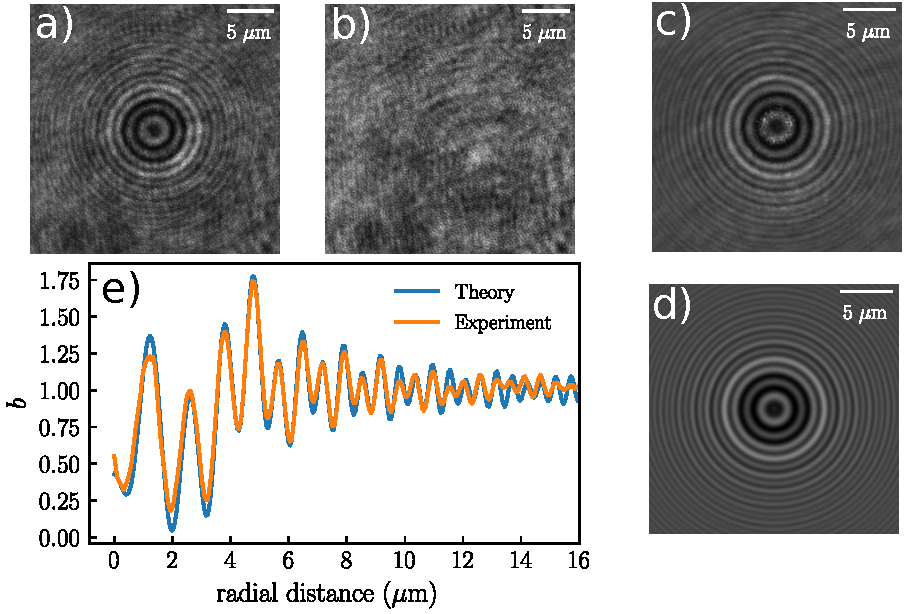
\includegraphics[scale=1]{02_body/chapter2/images/lorenz_mie_fit_demo/plot_lorenz_mie.pdf}
	\caption{a) Raw hologram of a $2.5 ~ \mathrm{\mu m}$ polystyrene particle measured experimentally with the setup detailed in section \ref{chap:exp-setup}. b) Background obtained by taking the median value of an image time series. c) Normalized hologram given by dividing a) by b). d) Result of the fit of c) using Eq.{\ref{Eq.normalized_Mie}}, from which the particle is found to be at a height $z = 14.77 ~ \mathrm{\mu m}$. e) Comparison of the normalized radial intensities, obtained experimentally from c) and theoretically from d).}
	\label{fig.Lorenz_mie_demo}
\end{figure}

\subsubsection{Hologram dependance on the particule's  characteristics}



As we can see with the Eq.\ref{Eq.Lorenz-Mie-function}, the in-line holograms vary with the position, radius and optical index of the particle. For in-line holograms, as both both incident and scattered field are collinear, the $x$ and $y$ positions of the particle are given by the center of the hologram. Thus, it is possible to track the motion of a colloid only in 2 dimensions by using algorithm such as the Hough transforms to find the center. As a side note, in that case, it would be optimal to place the particle just above the focal plane to have an Airy disk-like hologram, as shown in Fig.\ref{fig:holo_fix_n} for $a = 2.5 ~ \mathrm{\mu m}$ and $z = 5 ~\mathrm{\mu m}$.

\begin{figure}[H]
	\centering
	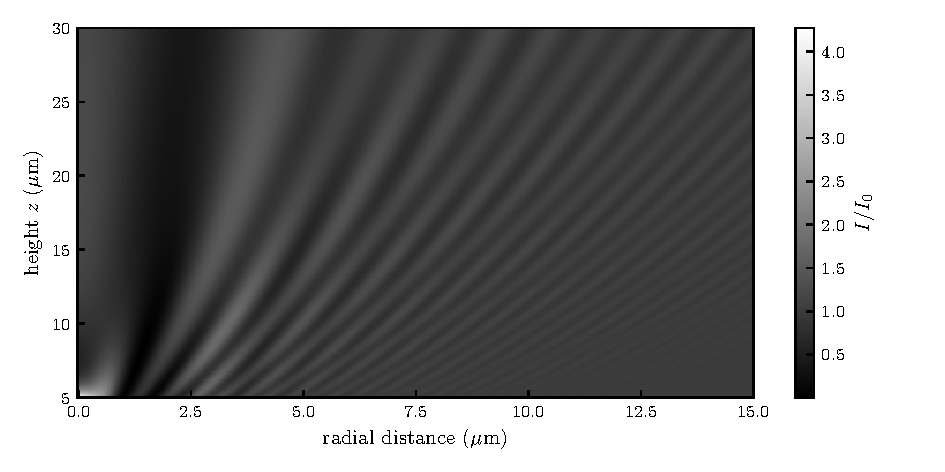
\includegraphics{02_body/chapter2/images/holo_size_exemple/holos_only_z.pdf}
	\caption{Hologram intensity map in the ($r,z$)-plan, calculated (see. Eq.~(\ref{Eq.normalized_Mie})) for a particle of radius $a = 1.5 ~\mathrm{\mu m}$ and optical index $n = 1.59$.}
	\label{fig:holo_onlyz}
\end{figure}

In order to gain some insights on how the holograms vary with the different parameters, one can compute theoritical (see. Eq.~(\ref{Eq.normalized_Mie})) holograms for particles of different sizes and heights. We start by considering a particle of radius $a = 1.5 ~ \mathrm{\mu m} $, and optical index $n_\mathrm{p}= 1.59 $ as shown in Fig.\ref{fig:holo_onlyz}. In this case, one can observe that as the distance $z$ between the particle and the focal plane increases, the hologram's rings get larger.

Additionally, this thickening of the rings can also be observed in the Fig.\ref{fig:holo_z_fit}, where hologram intensity profiles are plotted as a functions of the height $z$ both theoretically and experimentally for a polystyrene colloidal particle of radius  $a = 1.5 ~ \mathrm{\mu m} $, and for different couples of parameters in Fig.\ref{fig:holo_fix_n}.

Also, we note that if $z$ is not large enough compared to the radius of the particle, the center of an hologram can be so bright that the rings could not be seen if the camera does not have a large enough dynamic range.  Thus, for having an optimal condition for the fits, one should take care of defocusing enough the objective lens to have $z >> a$.





\begin{figure}
	\centering
	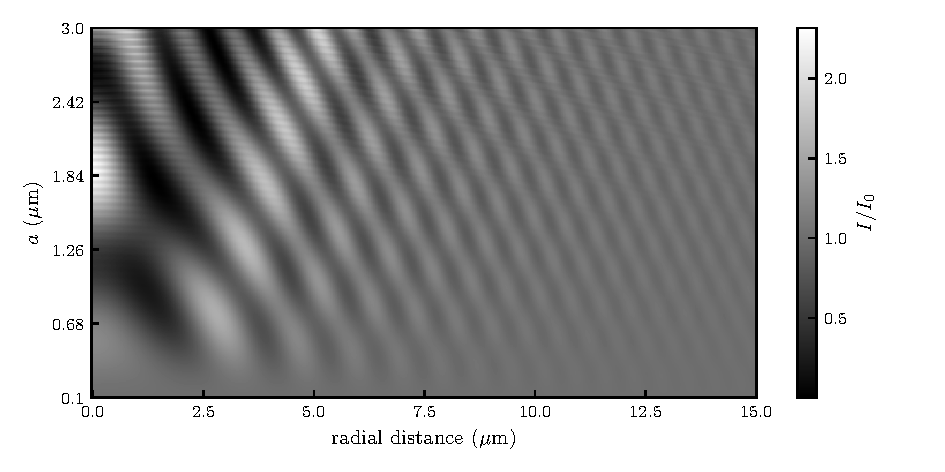
\includegraphics{02_body/chapter2/images/holo_size_exemple/holos_only_r.pdf}
	\caption{Hologram intensity map in the ($r,a$)-plan, calculated (see. Eq.~(\ref{Eq.normalized_Mie})) for a particle of optical index $n = 1.59$, and a distance $z = 15 ~\mathrm{\mu m}$ between the particle center and the focal plane of the objective lens.}
	\label{fig:holo_onlyr}
\end{figure}

\begin{figure}[H]
	\centering
	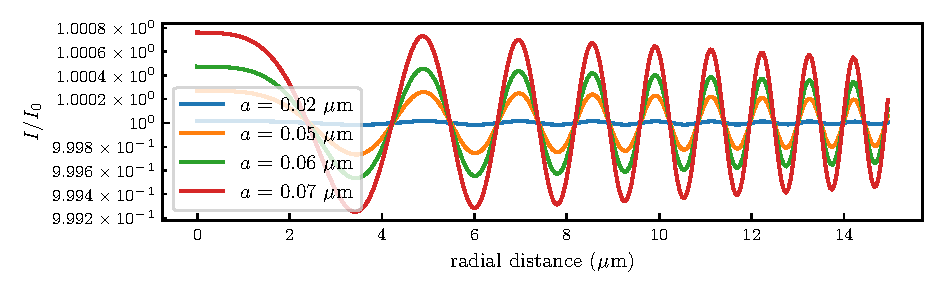
\includegraphics{02_body/chapter2/images/holo_size_exemple/smallparticles.pdf}
	\caption{Radial intensity profile for a the particle radius $a << \lambda$, and an optical index $n_\mathrm{p} = 1.59$ with a distance $z = 15 ~\mathrm{\mu m}$ between the particle center and the focal plane of the objective lens, and for a wavelength $\lambda = 532 ~ \mathrm{nm}$.}
	\label{fig:small_part_holo}
\end{figure}


We can now look at the holograms variation with respect to the radius of the particle as shown in Fig.\ref{fig:holo_onlyr} for a particle of optical index $n = 1.59$ and at a distance $z = 15 ~\mathrm{\mu m }$. One can observe that for small particles compared to the wavelength, \textit{i.e.} $a << \lambda$, we do not observe the rings. This is due to the fact that for the small particles, the scattering can be approximated using the Rayleigh theory in which the scattering is isotropic. Thus, the variation of intensity around $I_0$ will be smaller for smaller particles.

 Also, in this small-particle regime, the particle size does not affect the general shape of the hologram but just its intensity as shown in Fig.\ref{fig:small_part_holo}, for particles of radii between $a = 0.02 ~\mathrm{\mu m}$ and $a = 0.07 ~\mathrm{\mu m}$, and for a wavelength $\lambda = 532 ~\mathrm{nm}$.
 
  Additionally, since the signal-to-noise ratio is lower than for bigger particles, it is less precise to characterize small colloids compared to the wavelength.


 As the particle gets bigger, the scattering becomes anisotropic and is mostly oriented towards the incident plane-wave direction. This effect leads to an increase of the amplitude $I/I_0$ of the rings, as one can see in Fig.\ref{fig:holo_onlyr}. Thus, the signal-to-noise ratio is high enough to easily discern the hologram on top of the noise as one can see on the experimental picture of Fig.\ref{fig.Lorenz_mie_demo}-a). One who wants to use this method should thus use large enough particles for the hologram intensity to be greater than the camera noise level.



\begin{figure}[H]
	\centering
	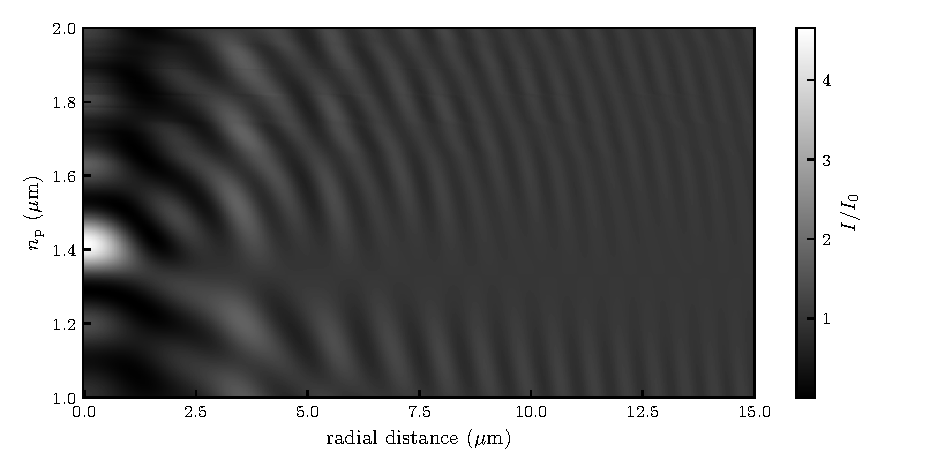
\includegraphics{02_body/chapter2/images/holo_size_exemple/holos_only_n.pdf}
	\caption{Hologram intensity map in the ($r,a$)-plan, calculated (see. Eq.~(\ref{Eq.normalized_Mie})) for a particle of optical index $n = 1.59$, and a distance $z = 15 ~\mathrm{\mu m}$ between the particle center and the focal plane of the objective lens.}
	\label{fig:holo_onlyn}
\end{figure}


Finally, one can check how the holograms are varying with the optical index of a particle. In this case, it is not the particle's optical index $n_\mathrm{p}$ which matters the most but the ratio $\zeta = n_\mathrm{p} / n_\mathrm{m} $ which can be found in the $a_n$ and $b_n$ formulas, in Eqs.\ref{Eq:an} and \ref{Eq:bn}. Indeed, for the scattering to happen, the optical index $n_\mathrm{p}$ of the colloid needs to be different from the optical index $n_\mathrm{m}$ of the surrounding medium. Additionally, the numerical solution of the Lorenz-Mie framework is not stable for $n_\mathrm{p} \simeq n_\mathrm{m}$. In Fig.\ref{fig:holo_onlyn}, we can observe holograms of a particle of radius $a = 1.5 ~ \mathrm{\mu m}$ at fixed distance $z=15 ~ \mathrm{\mu m}$ between the particle and the focal plane of the objective lens with a varying colloid's optical index, in water where $n_\mathrm{m} = 1.33$. In Fig.\ref{fig:holo_onlyn}, one can thus observe that for  $n_\mathrm{p} \simeq n_\mathrm{m}$ we do not see any holograms.  Additionally, one can observe that the signal-to-noise ratio gradually increases as $n_\mathrm{p}$ becones different from $n_\mathrm{m}$. One who wants to use this method should thus have $n_\mathrm{m}$ different enough from $n_\mathrm{p}$ for the hologram intensity to be greater than the camera noise level.






\subsubsection{Summary on the Lorenz-Mie method}

The combination of the height, optical index and radius of colloid thus gives unique holograms. This uniqueness of the holograms permits extracting precisely the position, optical index and radius of a colloid. In order to see how holograms are for different couples of parameters on the Figs.\ref{fig:holo_fix_z} and \ref{fig:holo_fix_n}, one can see possible holograms for different size and height. Additionally, one can use  the Jupyter Notebook on my github repository in order to plot any hologram \href{https://github.com/eXpensia/Ma-these/blob/main/02_body/chapter2/images/holo_size_exemple/holosize_variation.ipynb}{\faGithub}.  

Finally, Lorenz-Mie is the most versatile in-line holographic method, indeed, it permits tracking and characterize unique particles even without a priori knowledge. Besides, it is possible to write the Lorenz-Mie function $\vec{f}_\mathrm{s}$ for particular cases such as anisotropic \cite{fung_holographic_2013}, non-spherical particles \cite{wang_using_2014} or particle clusters \cite{fung_holographic_2013, perry_real-space_2013} to name a few; such possibilities open the door to a lot of experimental studies. Additionally, it can reach really high precision as the tenth of nanometer on the position and radius as well as $10^{-3}$ on the optical index \cite{lee_characterizing_2007}. 

Unfortunately, the Lorenz-Mie fitting suffer from a major drawback which is the time needed to fit one image. For example, a 200 by 200 pixels image, of a $2.5 ~ \mathrm{\mu m}$ particle's hologram, can take up to two minutes to be fitted using a pure and straightforward python algorithm. A lot of work as been done to have faster tracking, such as random-subset fitting \cite{dimiduk_random-subset_2014}, GPU (graphical processing unit) acceleration, machine-learning \cite{yevick_machine-learning_2014, hannel_machine-learning_2018} and deep neural networks \cite{altman_catch_2020}.

\begin{figure}[H]
	\centering
	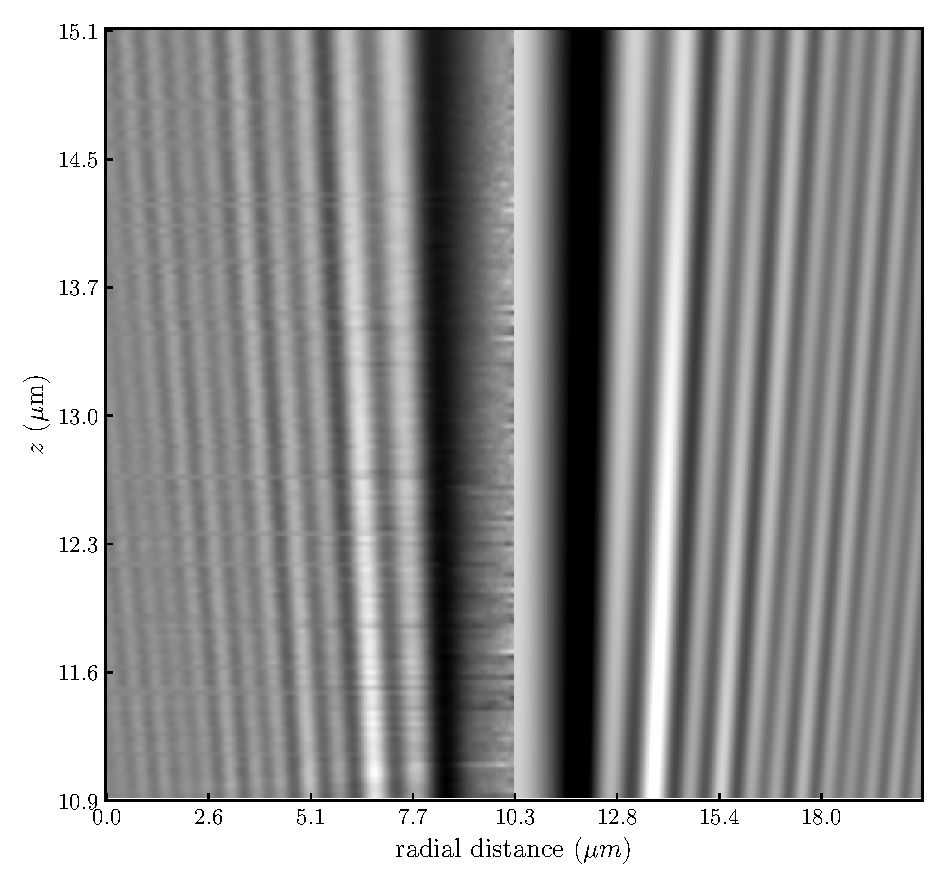
\includegraphics{02_body/chapter2/images/test_tableau2.pdf}
	\caption{On the left, experimentally measured  holograms' radial intensity profile stack, generated from a polystyrene bead of nominal radius $a = 1.5 \pm 0.035 ~ \mathrm{\mu m} $ using the experimental setup explained in chapter \ref{chap:exp-setup}. The calibration of this particle radius and optical index is shown in Fig.\ref{fig:KDErn}. On the right, the corresponding theoretical stack using the result of each individual hologram's fit.}
	\label{fig:holo_z_fit}
\end{figure}


\begin{figure}
	\centering
	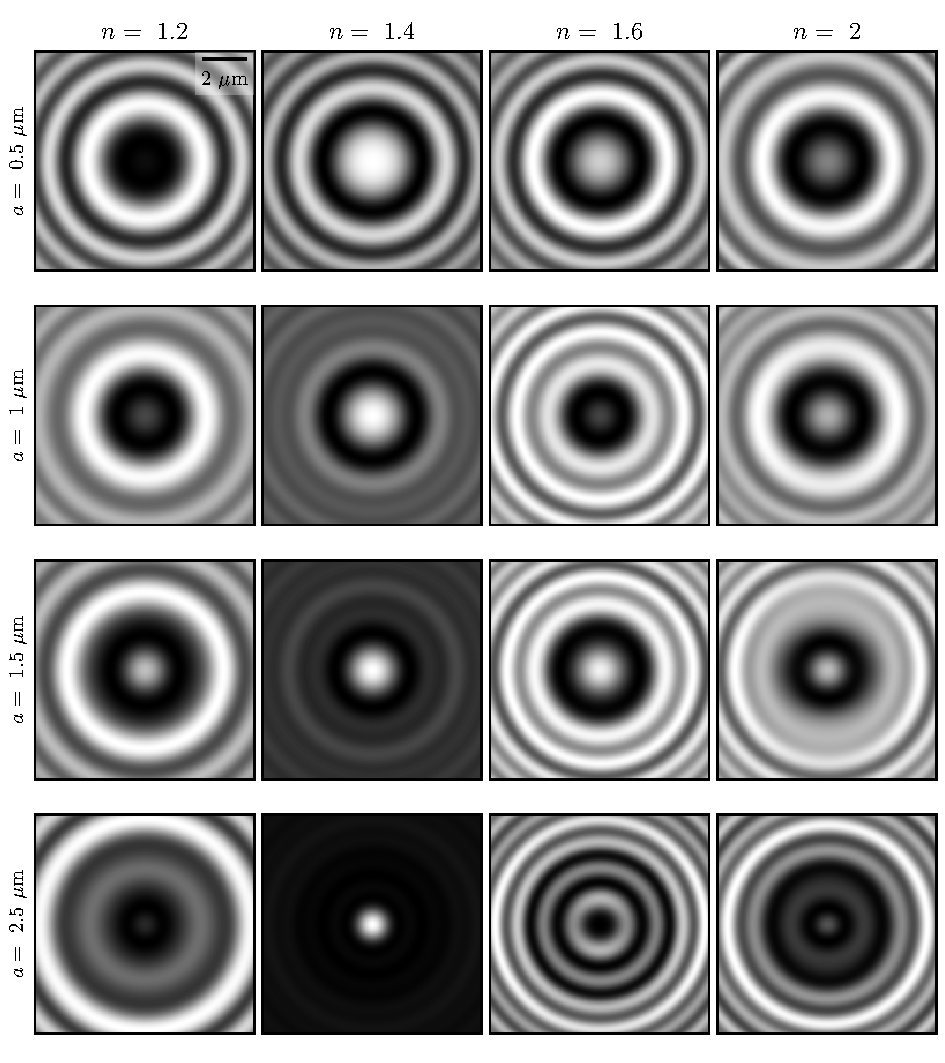
\includegraphics{02_body/chapter2/images/holo_size_exemple/holos_fix_z.pdf}
	\caption{On the left, experimentally measured  holograms' radial intensity profile stack, generated from a polystyrene bead of nominal radius $a = 1.5 \pm 0.035 ~ \mathrm{\mu m} $ using the experimental setup explained in chapter \ref{chap:exp-setup}. The calibration of this particle radius and optical index is shown in Fig.\ref{fig:KDErn}. On the right, the corresponding theoretical stack using the result of each individual hologram's fit.}
	\label{fig:holo_fix_z}
\end{figure}



\begin{figure}
	\centering
	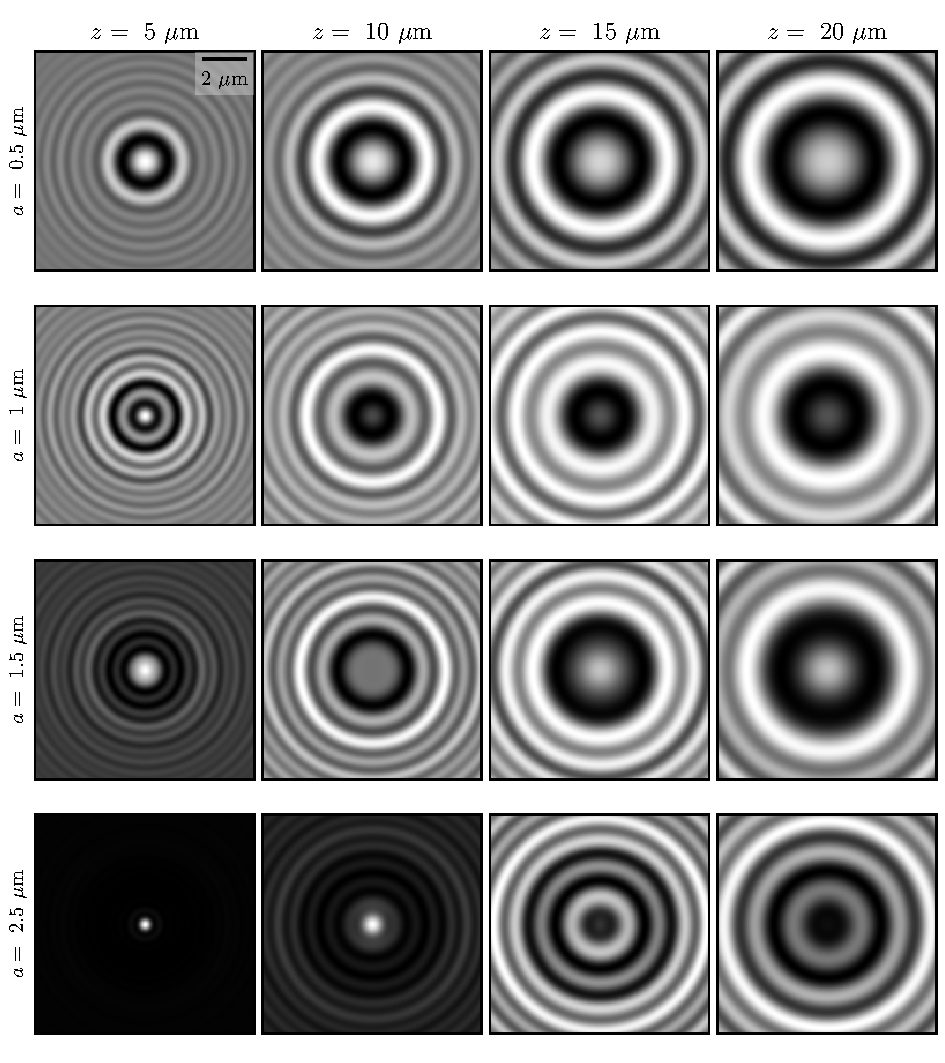
\includegraphics{02_body/chapter2/images/holo_size_exemple/holos_fix_n.pdf}
	\caption{On the left, experimentally measured  holograms' radial intensity profile stack, generated from a polystyrene bead of nominal radius $a = 1.5 \pm 0.035 ~ \mathrm{\mu m} $ using the experimental setup explained in chapter \ref{chap:exp-setup}. The calibration of this particle radius and optical index is shown in Fig.\ref{fig:KDErn}. On the right, the corresponding theoretical stack using the result of each individual hologram's fit.}
	\label{fig:holo_fix_n}
\end{figure}

\clearpage
\newpage

\subsection{Rayleigh-Sommerfeld back-propagation}





Rayleigh-Sommerfeld back-propagation \cite{wilson_3d_2012} works on the same principle as the Lorenz-Mie fitting but assumes that we have small scatterers, or, a low difference of optical index., such as :

\begin{equation}
	|\zeta - 1| << 1 \text{ and } ka|\zeta - 1| << 1 ~.
\end{equation}

In this case, at the focal plane, the intensity of the scattered field is smaller than the incident field, hence, the term $|\vec{E}_\mathrm{s}|^2$ can be ignored. Thus, the normalized intensity, Eq.\ref{Eq.normalized_Mie} can be rewritten as:

\begin{equation}
\frac{I(\vec{r})}{I_0(\vec{r})}= 1 + 2\Re \left( \frac{E_s(\vec{r},0)}{E_0(\vec{r})} \right) ~.
\end{equation}

If one can retrieve completely the scattered field from an image, it is possible to reconstruct it above the focal plane by convolution using the Rayleigh-Sommerfeld propagator \cite{goodman_introduction_2005}:

\begin{equation}
	h_{-z}(\vec{r}) = \frac{1}{2 \pi} \frac{\partial}{\partial z} \frac{\mathrm{e}^{ikR}}{R} ~,
	\label{Eq:propagator}
\end{equation}

where $ R^2 = r^2 + z^2 $ and the sign convention on the propagator indicates if the particle is below or above the focal plane. Using this propagator we have:

\begin{equation}
	E_s(\vec{r}, z) = E_z(\vec{r}, 0) \otimes h_{-z}(\vec{r})
\end{equation}

By using the convolution theorem \cite{cheong_strategies_2010, goodman_introduction_2005, sherman_application_1967,schnars_digital_1994} and supposing a uniform illumination, one can write the reconstructed scattered field at a height $z$ as:

\begin{equation}
	E_s(\vec{r}, z) \approx \frac{\mathrm{e}^{ikz}}{4\pi ^2}
	\int ^\infty _{- \infty}
	B(\vec{q}) H(\vec{q}, -z) \mathrm{e}^{i \vec{q} \cdot \vec{r}} d^2 q
	\label{Eq.RS} ~,
\end{equation}

where $B(\vec{q})$ is the Fourier transform of $I/I_0$ and $H(\vec{q}, -z)$ is given by

\begin{equation}
	H(\vec{q}, -z) = \mathrm{e}^{iz \sqrt{k^2 - q^2}} ~.
\end{equation}

Finally, using Eq.\ref{Eq.RS} one can reconstruct the scattered field and intensity since $I(\vec{r}) = |E_s(\vec{r})|^2$ as shown in Fig.\ref{fig.sommerfeld}. Moreover, by finding the position where we have an inversion of the center from bright to dark Fig.\ref{fig.sommerfeld}, we measure the position of the particle.
Those equations are way less computational intensive than the Lorenz-Mie function Eq.\ref{Eq.Lorenz-Mie-function}. Thus tracking can be way faster, moreover, Fourier transforms can be largely accelerated using GPU. 

Additionally, as the propagator Eq.\ref{Eq:propagator} take only into account the intensity of the image, this method does not require any information on the particle and number of particles. As a matter of fact,   to write Eq.\ref{Eq.RS}, one just need to assume that we have spherical colloids. Thus, this method is great to reconstruct the 3D position of a lot of particles or clusters formations. 

However, the major drawback is that it is the less precise of the presented measurements and that we can't use it to characterize the particles generating the holograms.




\subsubsection{Numerical Rayleigh-Sommerfeld back-propagation}

The \mintinline{python}{holopy} Python module also provide a set of method that permits to user the Rayleigh-Sommerfed back-propagation. Given the \mintinline{python}{hologram} variable containing all the needed metadata about the hologram such as the pixel size, medium index $n_\mathrm{n}$ illumination wavelength $\lambda$ and the actual image. Then, one can use the \mintinline{python}{propagate} method to back-propagate an hologram over a set of height \mintinline{python}{zstack} using the following Python snippet.

\begin{minted}
	[
	frame=lines,
	framesep=2mm,
	baselinestretch=1.2,
	fontsize=\footnotesize,
	linenos
	]
	{python}
	import holopy as hp
	import numpy as np
	
	zstack = np.linspace(0, 20, 11)
	rec_vol = hp.propagate(holo, zstack)
\end{minted}

Please note that using the \mintinline{python}{propagate}	 each propagation will be done by performing a convolution of the reference hologram over the distance to be propagated. However, better reconstruction can be obtained iteratively propagating holograms over short distance. The latter method is called Cascaded Free Space Propagation, and is particularly useful when the reconstructions have fine features or when propagating over large distances \cite{kreis_frequency_2002}. It can be done by specifying the argument \mintinline{python}{cfsp} to the  \mintinline{python}{propagate} method. For example, to propagate three steps over each distance, we can use \mintinline{python}{hp.propagate(holo, zstack, cfsp=3)}.



\begin{figure}[!ht]
	\centering
	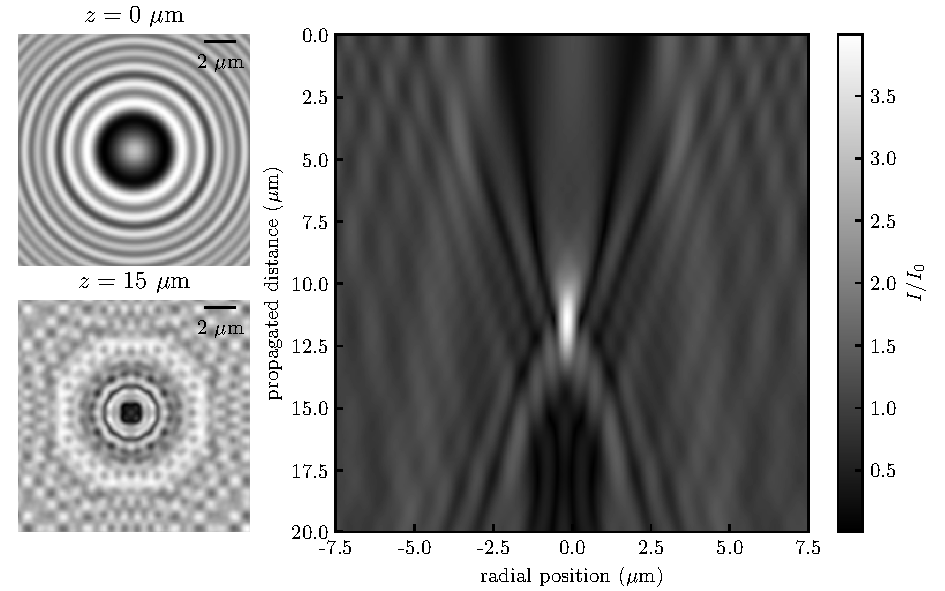
\includegraphics{02_body/chapter2/images/Back-propagation/backpropagation.pdf}
	\caption{On the left: the original hologram on the top and propagated along $15 ~ \mathrm{\mu m}$ on the bottom. On the right: Reconstruction using Eq.\ref{Eq.RS} of the scattered intensity of single colloidal sphere of a radius $a = 0.1 ~ \mathrm{\mu m}$  polystyrene spheres, $n_\mathrm{p} = 1.59$ in water at a originalm $n_\mathrm{m} = 1.59$, height of $15 ~ \mathrm{\mu m}$.}
	\label{fig.sommerfeld}
\end{figure}



\subsection{Experimental setup}
\label{chap:exp-setup}

The experimental setup I used during my PhD could be employed in order to use both Lorenz-Mie and Rayleigh-Sommerfeld Back progation methods. In order to observe the holograms we use an homemade inverted microscope as shown on the Fig.\ref{fig:picture} and shematized in Fig.\ref{fig:schema}. This microscope is built using Thor Labs cage system, as it permits doing vertical construction easily. Using this microscope, we observe the holograms coming form the interactions between a laser sourced and the beads present in a sample.

A sample consists of a parallelepipedic chamber ($1.5 ~ \text{cm} ~ \times ~ 1.5 ~ \text{cm} ~ \times ~ 150 ~ \mathrm{\mu m} $), made from two glass covers, a parafilm spacer, and sealed with vacuum grease, containing a dilute suspension of spherical polystyrene beads. Sealing the sample with vacuum grease permits to drastically decrease the evaporation, this permits to reduce the possible evaporation driven flow in the sample.

We used 3 different colloidal sizes, of nominal radii $0.56 ~ \mathrm{\mu m}, ~ 1.5 ~ \mathrm{\mu m} \text{ and } 2.5 ~ \mathrm{\mu m} $, at room temperature $T$, in distilled water (type 1, MilliQ device) of viscosity $\eta = 1 ~ \mathrm{mPa.s}$. The particles are made of polystyrene of density $\rho = 1050 \mathrm{kg.m^{-3}}$ and optical index $n_\mathrm{p} = 1.598$ for a wavelength of $532$ nm.

 The sample is illuminated by a collimated laser beam with a $532$ nm wavelength. The used laser delivers a power of 4 W and has a centimetric waist. Since the laser is collimated, it has a near zero exentricity such as it can be seen as a plane wave. With this characteristics, we can assume that there is no optical force exerted on the particles [NEED TO CHECK HOW TO EVALUATE THAT]. As depicted in the chapter \ref{chap:LM_fit}, the light scattered, by one colloidal particle at a given time $t$, interferes with the incident beam. 
 
 An oil-immersion objective lens (x60 magnification, $1.30$ numerical aperture) collects the resulting instantaneous interference pattern, and relays it to a camera (Basler acA1920-155um) with a $51.6$ nm/pixel resolution (see Fig.\ref{fig.Lorenz_mie_demo}a)). 
 
 The exposure time of the camera is set to $\tau_{\mathrm{expo}} = 3$ ms to avoid motion-induced blurring of the image. As a general rule, the particle should not diffuse more than the pixel size during that time, such that here $2D\tau_{\mathrm{expo}} < 51.6$ nm.

\begin{figure}[!ht]
	\centering
	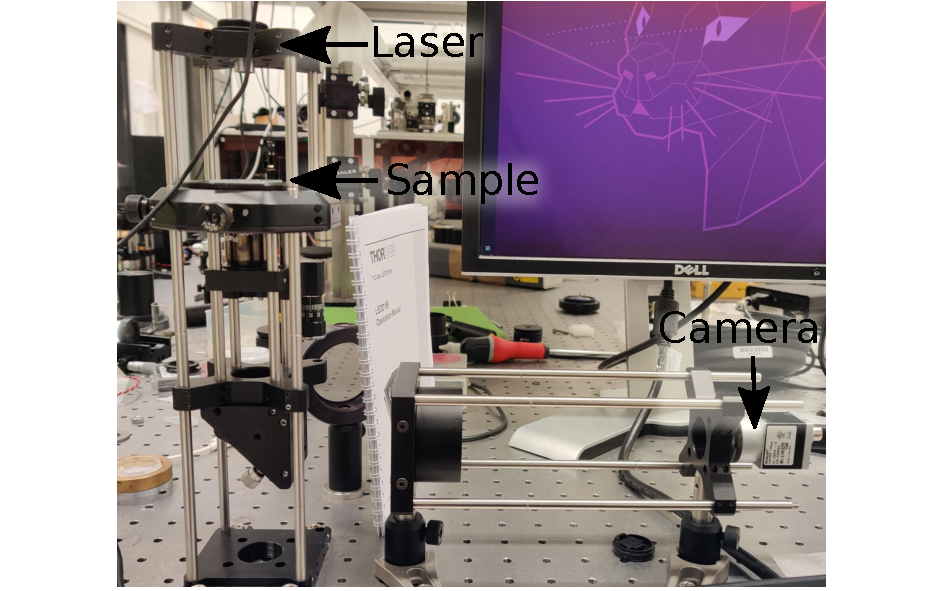
\includegraphics{02_body/chapter2/images/figures_setup/photo_setup.pdf}
	\caption{Photo of the custom build microscope used along my thesis. It is mainly composed of Thorlabs cage system. The camera used is a Basler acA1920-155um, we use a x60 magnification and $1.30$ numerical aperture oil-immersion objective lens. The light source is a colimated  $521 ~ \mathrm{\mu m}$ wavelength laser.}
	\label{fig:picture}
\end{figure}

\begin{figure}[!ht]
	\centering
	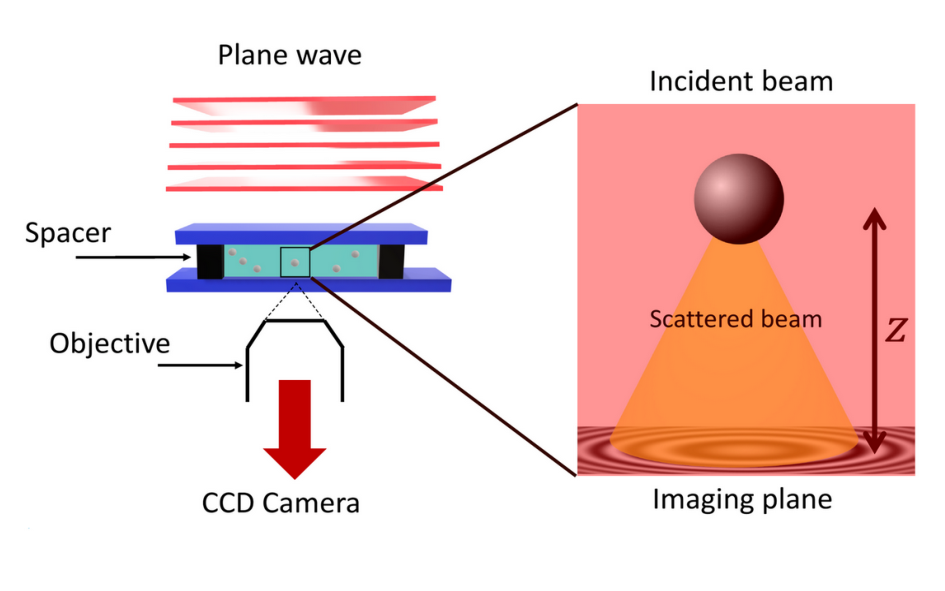
\includegraphics[scale=0.9]{02_body/chapter2/images/figures_setup/schema_setup.pdf}
	\caption{Schematic of the experimental setup. A laser plane wave of intensity $I_0$ illuminates the chamber containing a dilute suspension of micro-spheres in water. The light scattered by a particle interferes with the incident beam onto the focal plane of an objective lens, that magnifies the interference patten and relays it to a camera.}
	\label{fig:schema}
\end{figure}


\subsection{Optical forces}

As we illuminate the particle with a laser, it is important to know if the optical forces that arises from the interactions between the light and the particle needs to be taken into account. When a plane wave is incident on a sphere, it scatters and absorbs light. This process depends both on the light wavelength $\lambda$ and on the sphere properties, its radius $a$ and refractive index $n_\mathrm{p} = n_{r} - jn_i$. As for polystyrene the imaginary part $n_i \ll 1$ as shown in Fig.\ref{fig:refractive_index} we neglect it, however, since we want here compute the optical forces, and hence, the quantity of the light which is absorbed we will consider it in this section. Additionally, in the Mie theory, the particle is characterized by the size parameter $\tilde{x}= 2\pi a /\lambda$. The optical force $F_\mathrm{opt}$ is given by \cite{f_bohren_absorption_1998}:

\begin{equation}
	F_\mathrm{opt} = \frac{I_\mathrm{r} n_\mathrm{m} \pi a^2 }{c} (Q_\mathrm{ext} - gQ_\mathrm{sca}) ~,
	\label{Eq.Fopt}
\end{equation}

where $I_r$ is the irradiance in $\mathrm{W.m^{-2}}$ on the sphere,  $c$ is the speed of light in vacuum, $g=\pi r^2$ the sphere cross section and  $Q_\mathrm{ext}$ and $Q_\mathrm{sca}$ being respectively the extinction and scattering efficiency given by:

\begin{equation}
	Q_\mathrm{ext} = \frac{2}{k^2 a^2} = \sum _{n=1} ^\infty (2n + 1 ) (|a_n|^2 + |b_n|^2) ~,
\end{equation}

and,

\begin{equation}
	Q_\mathrm{ext} = \frac{2}{k^2 a^2} = \sum _{n=1} ^\infty (2n + 1 ) \Re (a_n + b_n) ~,
\end{equation}

where the $a_n$ and $b_n$ coefficient are given by the Eqs.\ref{Eq:an} and \ref{Eq:bn} respectively.


\begin{figure}[H]
	\centering
	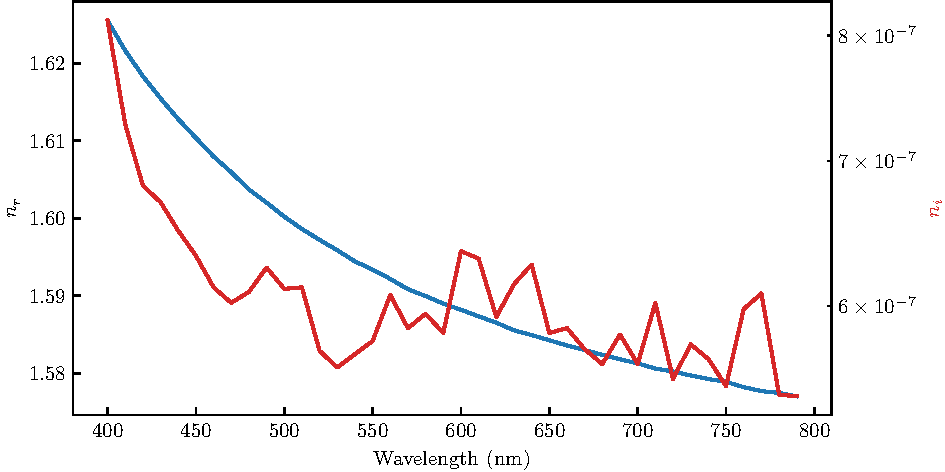
\includegraphics[scale=0.9]{02_body/chapter2/images/Calcul_force_optique/refractive_index.pdf}
	\caption{Real (left axis) and imaginary (right axis) part of the refractive index of polystyrene as a function of the incident wavelength. Data obtained from \cite{zhang_complex_2020}}
	\label{fig:refractive_index}
\end{figure}

To compute the optical force I personally use the \mintinline{python}{miepython} python's module \href{https://github.com/scottprahl/miepython/}{\faGithub} and retrieving the optical index data using the \href{https://refractiveindex.info/?shelf=organic&book=polystyren&page=Zhang}{refractiveindex.info} website, using the following Python snippet.

\begin{minted}
	[
	frame=lines,
	framesep=2mm,
	baselinestretch=1.2,
	fontsize=\footnotesize,
	linenos
	]
	{python}
import miepython as mp
import numpy as np

# Download the data on the refractiveindex.info website
poly = np.genfromtxt(
r"https://refractiveindex.info/tmp/data/organic/(C8H8)n%20-%20polystyren/Zhang.txt",
delimiter="\t",
)
N = len(poly) // 2
poly_lam = poly[1:N, 0]  # wavelength
poly_nre = poly[1:N, 1]  # real part
poly_nim = poly[N + 1 :, 1]  # imaginary part

x = 2 * np.pi * a / poly_lam
n = poly_nre - 1.0j * poly_nim
qext, qsca, qback, g = mp.mie(n, x)  # compute the efficiencies
E0 = 4.5e-3 / (np.pi * 1.75e-3 ** 2)  # compute the irradience
c = 299792458 / 1.33  # light velocity in the  medium

F = E0 * np.pi * r0 ** 2 * (qext - g * qsca) / c  # compute the optical force

\end{minted}

\begin{figure}[H]
	\centering
	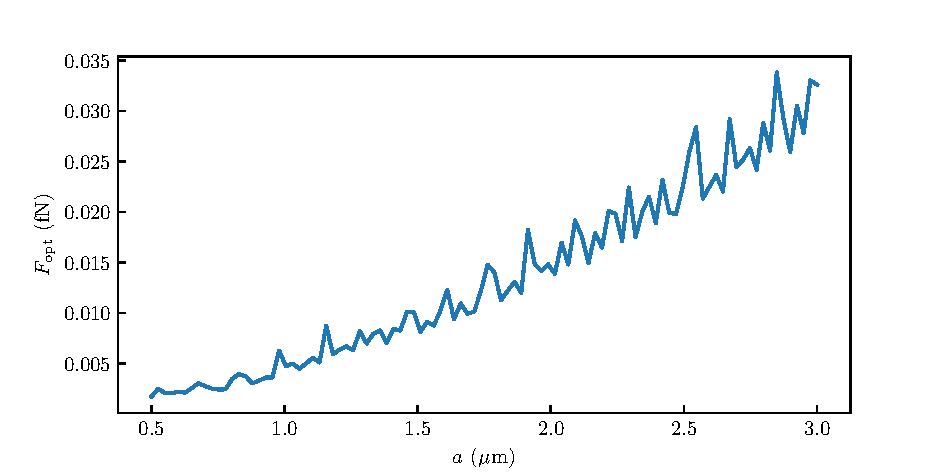
\includegraphics[scale=0.9]{02_body/chapter2/images/Calcul_force_optique/optical_force.pdf}
	\caption{Optical force $F_\mathrm{opt}$ (see Eq.\ref{Eq.Fopt}) exerted on a spherical particle of radius $a$ by a plane wave of wavelength $\lambda = 532$ nm, and of irradiance $I_\mathrm{r} = 467.7 ~ \mathrm{W.m^{-2}}$. The force is computed using the \mintinline{python}{miepython} python's module \href{https://github.com/scottprahl/miepython/}{\faGithub} and the refractive index of polystyrene \cite{zhang_complex_2020}.}
	\label{fig:optical_force}
\end{figure}

Using Python, one can thus compute the optical force $F_\mathrm{opt}$ as a function of the particle radius. As shown on Fig.\ref{fig:optical_force} the optical exerted on the colloidal particle from the microscope's illumination source, is of the order of magnitude $F_\mathrm{opt} \simeq 10^{-2}$ fN. By comparing this result with the buoyant of a colloidal particle $F_\mathrm{g}$:

\begin{equation}
	F_\mathrm{g} =  \frac{4}{3} \pi (\rho_\mathrm{m} - \rho_\mathrm{p}) g ~,
\end{equation}

we found that for a particle of radius $a = 0.5 ~\mathrm{\mu m}$, $F_\mathrm{g} = -0.3 $ fN and for $a = 1.5 ~\mathrm{\mu m}$, $F_\mathrm{g} = -7 $ fN. Thus, we can conclude that $F_\mathrm{opt} \ll F_\mathrm{g}$, hence, in the following of the manuscript we neglect the optical force as it is lower than the other external forces acting on the colloids. Howver, experiments on Brownian motion with has been done by increasing the irradiance to $10^6 ~\mathrm{W.cm^{-2}}$ an they were able to measure the optical force from the motion statistics \cite{prieve_measurement_1999}.




\subsection{Experimental pipeline}
The method we choose is the Lorenz-Mie fitting method, since this it permits the characterization of single particles. Indeed, since we are interested to fine effects near the surface, we need to know perfectly the radius of the particle we have recorded. This feature also make our all process calibration free, as we don't need to assume any physical properties. An exemple of the pipeline that pemits to track a single particle trajectory is shown in the appendix \ref{app:tracking}. In the following, the different steps of the pipe line are going to be described.

\subsubsection{Recording the holograms}
Since we use a Basler camera, we use the provided Pylon software in order to record the holograms. The latter permits to adjust the parameters of the camera, such as the region of interest (\gls{ROI}), frames per second (\gls{fps}) or the opturation time to name a few. Also, movies can be recorded as a time series of images, AVI or MP4 files. AVI files or times series are a great way to save the movies since they are lossless. However, in general we use an \gls{ROI} of $1000 \times 1000$ pixels to record the particle for a long time enough. 


Additionally, since the recording is done using 8 bits per pixel (or 256 gray levels), an image of $1000 \times 1000$ pixels needs a disk space of $1$ MB \footnote{An uppercase B denotes Byte which is equivalent to 8 bits, such as $1\mathrm ~ {B} = 8 ~ \mathrm{b}$. For storage indications, Bytes are generally used, since historically a set of $8$ bits encodes a single text character, and, are for this reason the smallest addressable memory unit in most of the computer architectures. As an example, in binary ``LOMA" would be encoded by ``01001100 01001111 01001101 01000001" }. One can thus see that image sequences and AVI files are not suitable for our case because of several points: i) at $100$ \gls{fps} one would need $108 ~ \mathrm{GB}$ to store a 30 minutes film, it could lead to TB of data per experiment which was not manageable. ii) it would require a sequential writing speed of 60 $\mathrm{MB/s}$, which is just below the limit of the better HDD. iii) AVI files are bound to 2 GB maximum thus dramatically reducing the length of the experiments.

To conclude, for all of these reasons, we choosed to use the MP4 files format (MPEG-4 encoding) for the video recording. Using the lowest compression, we did not observe any impact on the fitting process due to quality loss. Finally, a video of 30 minutes will size $\simeq 3$ GB.


\subsubsection{Fitting the holograms}


Once the holograms are recorded, we fit all of the images to retrieve the trajectory of the particle. To do so, we choosed to use the Pylorenzmie module developed by the Grier's lab at the New York University. Although this module present a lot of capabilities, it is quite cumbersome to use, thus, I developed a wrapper around the module that I called wraplorenzmie which can be found on my github repository \href{https://github.com/eXpensia/wraplorenzmie}{\faGithub}. 

This wrapper permits to directly load the MP4 files, compute the background and choose if what parameters should be fitted. While fitting a series of images, it uses the results of the previous image as the initial fit parameters.

However, as presented in the section \ref{chap:LM_fit} about the Lorenz-Mie fitting, the main drawback is the time to fit an image. Indeed, using a Python algorithm, one needs $30$ seconds to fit images of $100 \times  100$ pixels and a few minutes for a $500\times 500$ pixels hologram. We can directly see a bottleneck, indeed, if one want to track one trajectory made of $100~000$ images one would need to wait a minimum of $\simeq 70$ days; for a series of images that need only a few minutes to be shot experimentally. 

When I started my PhD, two groups, the Grier's lab and the Manoharan's lab, had already introduced python packages, respectively, Pylorenzmie and Holopy in order to inverse holograms. They had introduced ways to only fit a set of randomly chosen pixels, and, demonstrated that taking only $1~\%$ of the image pixels, could lead to similar precision and improve considerably the fit's execution time \cite{dimiduk_random-subset_2014}.
 
 Unfortunately, even if fitting  a random subset of pixels is faster, it leads to a few images per second, and, is still too long for the amount of data we wanted to have. Ironically, this part of my project is certainly the one where I spent the most my time, and I certainly learned a lot about code optimization and computer cluster usage. 
 
 It is around the half of my thesis, that Pylorenzmie got a new commit on their github repository which was telling that they succeeded on using GPU acceleration using CUDA\footnote{CUDA is the acronyme of Compute Unified Device Architecture. It is a parallel computing platform and programming model made to permits an easier use the GPU for general purpose. CUDA is developed by NVIDIA since 2012, thus all recent NVIDIA's GPUs are CUDA enable. It is possible to use it with every language as long as a library as been developed, such as cupy for Python \href{https://github.com/cupy/cupy}{\faGithub}.}. This was not an easy task since they needed to reconstruct the Bessel functions in an understandable way for the GPU, fortunately it is possible to do so by using continued fractions \cite{lentz_generating_1976}. This humongous update permits fitting whole images at a whooping speed improvement of 20 fps. At this speed, we fit the tridimension position of the particle, the radius and optical index. 
 
 As a remark, the fits are done by soliving a least square problem using the Levenberg-Marquardt algorithm \cite{more_levenberg-marquardt_1978}. This algorithm, is largely used in any curve-fitting applications due to it capabilities to find a minimum even by starting far from it. As mentionned, it is also possible to use various models of Machine Learning or Deep Learning to do the fits \cite{altman_catch_2020}. However since we can write analyticaly the holograms, the deep learnings models can't be more precise than a standard least-square fitting process. Deep Learning however, could be a great option is one wants to prioritize the computation time over the fit's precision.
 
 
 Finally, to have a more reliable and fast tracking, we beggin by fitting the first $10~000$ with  $\vec{r}_\mathrm{p}$, $a$ and $n_\mathrm{p}$ as free parameters. Using the results of this fit we can characterize the physical properties the observed colloid with high precision. Then, using the later result we can fit all the images with only the particle position $\vec{r}_\mathrm{p}	$ as a free parameter.
 



\subsubsection{Radius and optical index characterization}
\label{sec:radius_charac}

Once the data of the radius and optical index retrieved, the quantity we can look at is the the distribution of measurements. Using $10 ~ 000$ measurements one can do a 2D histogram of the $a$ and $n_\mathrm{p}$ as presented in the fig.\ref{fig:KDErn} here smoothed using a Gaussian KDE (Kernel Density Estimator). Using the later using the top 10\% measurements couple possibility, we measure that the radius of the observed particle is $a=1.514 \pm 0.003 ~ \mathrm{\mu m} $ and its optical index $n_\mathrm{p} = 1.585 \pm 0.002$.
 




Finally, using this measurement of radius and optical index, we fit the whole movie by removing them from the free parameters. Doing so, we have measured the trajectory of the particle as shown in Fig.\ref{fig:3dtrajec} in tridimension for the particle previously characterized.

\begin{figure}[!ht]
	\centering
	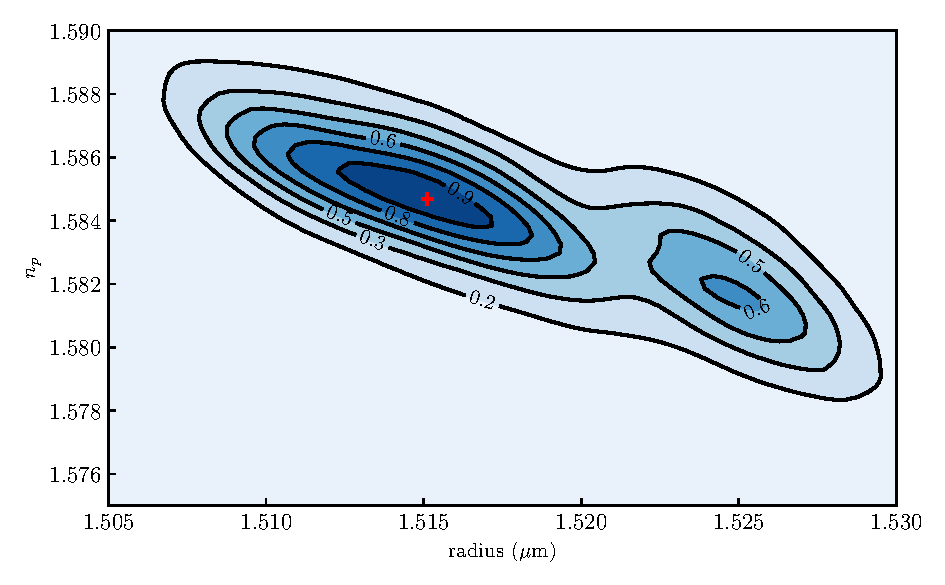
\includegraphics{02_body/chapter2/images/KDErn.pdf}
	\caption{2D Probability density function of the measurements of the optical index $n_\mathrm{p}$ and radius $a$. Black lines indicate iso-probability. Taking the $10\% $ top probability, we measure $n_\mathrm{p} = 1.585 \pm 0.002$ and $a=1.514 \pm 0.003 ~ \mathrm{\mu m}$. }
	\label{fig:KDErn}
\end{figure}

\begin{figure}[H]
	\centering
	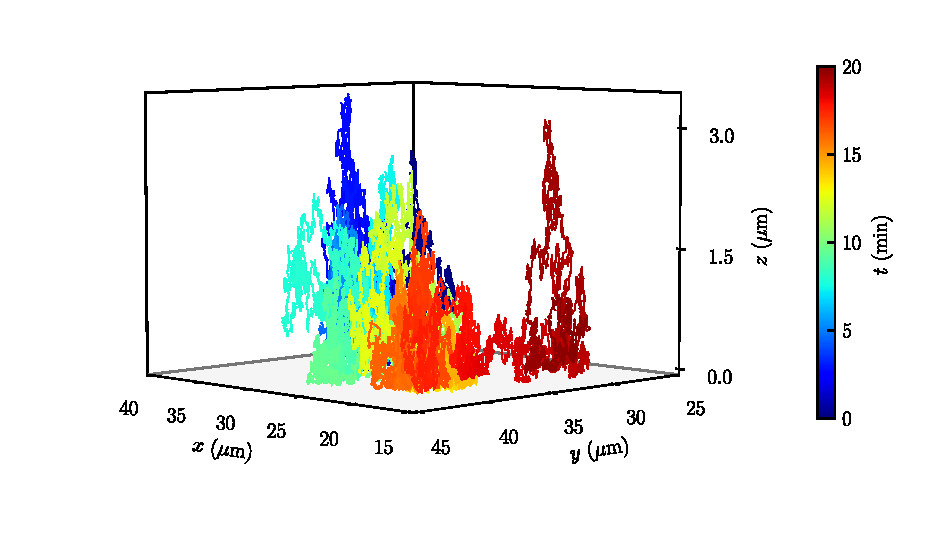
\includegraphics{02_body/chapter2/images/trajectory/traj.pdf}
	\caption{3D plot of an experimental trajectory measured in water for a particle of optical index $n_\mathrm{p} = 1.585$ and radius $a = 1.514  ~ \mathrm{\mu m}$.}
	\label{fig:3dtrajec}
\end{figure}

\subsubsection{Conclusion}

In this chapter, we have covered different method that enable the tracking of individual particles. All the different method each come with pros and cons. We decided to use Lorenz-Mie since it is requires no calibration. Then we have shown how we use it in practice, from the experimental setup to the numerical treatment. Also, an exemple of the Jupyter notebooks used for the traking can be found in the appendix \ref{app:tracking}.  We have discussed on how to have fast and accurate fits to retrieve the particle trajectory. To do so, we first characterize fully the particle, namely, its radius and optical index; before tracking a whole movie. 

Now that we have an understanding on the tracking of single colloids, we can use the later measured trajectory in order to understand how the Brownian motion is affected in various configurations. In the following, use confined Brownian motion in order to do a stochastic inference of surface-induced effects.
